
%%%%%%%%%%%%%%%%%%%%%%%%%%%%%%%%%%%%%%%%%%%%%%%%%%%%%%%%%%%%%%%%%%%%%%%%%%%%%%%
%
% Nicole's Thesis, IIT 2018
%
%%%%%%%%%%%%%%%%%%%%%%%%%%%%%%%%%%%%%%%%%%%%%%%%%%%%%%%%%%%%%%%%%%%%%%%%%%%%%%%
\documentclass{iitthesis}

% Document Options:
%
% Note if you want to save paper when printing drafts,
% replace the above line by
%
%   \documentclass[draft]{iitthesis}
%
% See Help file for more about options.

\usepackage[dvips]{graphicx}    % This package is used for Figures
\usepackage{rotating}           % This package is used for landscape mode.
\usepackage{epsfig}
\usepackage{subfigure}          % These two packages, epsfig and subfigure, are used for creating subplots.
%\usepackage{siunitx}

%% Only for editing process...TAKE OUT for FINAL DRAFT
\usepackage{graphicx,xcolor,enumitem}
\newcommand{\lsnote}[1]{\textsf{{\color{violet}{ LS note:}   #1 }}}
\newcommand{\nrnote}[1]{\textsf{{\color{blue}{ NN note:}   #1 }}}
\newcommand{\jpnote}[1]{\textsf{{\color{green}{ JP note:}   #1 }}}

\begin{document}

\title{Design for Staged Two Beam Acceleration at the Argonne Wakefield Accelerator Facility}

\author{Nicole Neveu }
\degree{Doctor of Philosophy}
\dept{Physics}
\date{May 2018}
\copyrightnoticetrue      % crate copyright page or not
%\coadvisortrue           % add co-advisor. activate it by removing % symbol to add co-advisor
\maketitle                % create title and copyright pages


\prelimpages         % Settings of preliminary pages are done with \prelimpages command

%%%  Acknowledgement %%%
\begin{acknowledgement}     % acknowledgement environment, this is optional
	\par  Family, Lalo, Linda, John, AWA group, Jeff
	%\input{ackno.tex} % you need a separate acknowledgement.tex file to include it.
\end{acknowledgement}

% Table of Contents
\tableofcontents
\clearpage

% List of Tables
\listoftables

\clearpage

%List of Figures
\listoffigures

\clearpage

%List of Symbols(optional)

\listofsymbols
\SymbolDefinition{$c$}{Speed of Light}
\SymbolDefinition{$\epsilon$}{Dielectric Permittivity}
\SymbolDefinition{$\epsilon$}{6D Phase Space Emittance}
\SymbolDefinition{$\gamma$}{Relativistic Kinetic Energy}

\clearpage

%%% Abstract %%%
\begin{abstract}           % abstract environment, this is optional
	\par Staged two beam acceleration using dielectric structures has yet to 
	be achieved anywhere in the world. In this thesis, I discuss the beam 
	line design and simulation, followed by experimental results of a 
	beam line with the potential for dielectric TBA.   
\end{abstract}

\textpages     % Settings of text-pages are done with \textpages command

\Chapter{INTRODUCTION}

\Section{Motivation} \label{sec:motivation}

If there is ever a new generation of accelerators dedicated to High Energy Physics
(HEP), they will be of the TeV scale. Reduction in the size and cost
of such machines is key to their feasibility, and can be accomplished
through accelerator technology R\&D. Investigation into a 
high gradient candidate for future HEP machines was underway
at the Argonne Wakefield Accelerator (AWA) facility. A
short pulse, two-beam acceleration (TBA) scheme using 
wakefield power extractors, and accelerating structures made 
of metallic materials was designed. 
The goal of AWA is to demonstrate a gradient of
%\SI{250}{MV/m}, using a TBA dielectric scheme. If successful, this would
be the only facility in the world capable of such gradients used for
acceleration of a beam.

Despite the advantage of higher gradients, there is still experimental work
needed to prove dielectric TBA is a viable candidate for implementation at an HEP or user facility.
TBA requires a drive beam to pass through a decelerating structure and
lose energy through wakefield generation. The electromagnetic wake
is coupled from the decelerator into an accelerating structure, where
the electric field is used to accelerate a second beam. This requires
two complete and separate beamlines operating synchronously with each other.  
The wakefield structures can be metallic or dielectric. Dielectric
structures, having no irises, are simple to manufacture and have demonstrated
%high gradient capability at \SI{100}{MV/m} \cite{WeiPaper}. 

The Compact Linear Collider (CLIC) collaboration, proposes a similar TBA scheme with
%a \SI{240}{ns} pulse design. This limits the acceleration gradient
%to roughly \SI{150}{MV/m} at room temperature due to rf breakdown \cite{CLICdesignReport}.
Higher gradients could be reached when driven by a very short drive
beam pulse, such as the 20ns pulse length proposed by AWA \cite{WeiPaper}. 
\nrnote{Understand and explain why short pulse can give higher gradients. 
Because higher peak power is tolerable, but average power stays the same?}
While the two groups vary on approach, it is agreed that TBA would 
require less infrastructure when constructing a linear TeV scale machine, 
versus the cost of more conventional technology. 
%For example, a case study was done using traditional \SI{50}{MW} klystron sources.
It would take roughly 35,000 klystrons to construct a linear machine to deliver the same 
%\SI{9.2}{TW} power specification in CLIC reports \cite{CLICdesignReport}. 
%In comparison to CLIC's 48 km projected length to reach \SI{3}{TeV}, the Next Linear
%Collider (NLC) collaboration projected a length of \SI{26}{km} using X-band klystrons,
%only to reach an energy of \SI{1}{TeV}. %\cite{NLC}. 
The power supplied to the witness beam in TBA is similar to
power provided by traditional accelerator technology. 
The key difference is the amount of infrastructure and cost 
needed to transport the power. Theoretically, TBA can deliver
the same amount of power as conventional methods with less 
infrastructure, and therefore lower cost, in the case of a high energy machine. 

Before a true study of the power and infrastructure trade offs 
can be done, the feasibility of staged TBA must be understood, 
as no high energy machine can be built with out a staging.
Staging is the ability to use two accelerating modules back to back to accelerate 
the same particle bunch. While simple in principle, the difficulties 
to achieve staging should not be underwritten. Demonstration of staging proves 
that a TBA scheme can be scaled to high energies, and whether it is 
feasible to use such methods. Single stage TBA, and staging 
in a simplified scheme have been demonstrated at the AWA in 2016.
\nrnote{Not any more? - Demonstration of the full-scale dielectric staging scheme is the 
	subject of this thesis.} 
Desing and partial testing of a full-scale staging scheme is the 
subject of this thesis. The branched drive beam line was designed and 
simulated. 
Optimization of the bunch train timing took place, \nrnote{not? - the two 
	beam lines were synchronized and experimental measurements 
	of staged TBA were taken. }
Experimental results and comparison to simulations, along 
with the following beam dynamics analysis is shown here.

\Section{Argonne Wakefield Accelerator Facility} \label{sec:facility}

% \lsnote{testing this }
The AWA facility consist of two rf photoinjector electron guns operating
%at \SI{1.3}{GHz}, and three subsequent beam lines. %\cite{AWAlayout}. 
Two of the beam lines are currently used for staged TBA, and the
third is used for Emittance Exchange experiments (EEX). A layout of
the facility is shown in Fig. \ref{fig:bunker}. 

The beam line located on the right side of Fig. \ref{fig:bunker} is called the
drive line. The rf photoinjector on the drive line uses a semiconducting
CsTe cathode, and is followed by a linear accelerator (linac). The
drive linac uses six copper cavities and four klystrons to accelerate the drive beam
%to energies of 50-\SI{70}{MeV}. The number of bunches generated from each 
laser pulse can vary from 1, 2, 4, 6, and 8 bunches. When multiple bunches
are generated, the grouping is called a bunch train. Generation of
these variable bunch trains is accomplished by splitting the pulsed
UV laser beam before it enters the gun and hits the cathode. The splitting
takes place in a complex network of UV optics located near the drive
gun. The optics set up is called a beam splitter, or mulitsplitter,
%and trains are created at a rate of 0.5, 1, or \SI{2}{Hz}. This timing is
called a pulse, or the repetition rate of the machine. A picture of
the AWA multisplitter table is shown in Fig. \ref{fig:optics}. Optimization 
of the UV optics was performed and is detailed in Section \ref{sec:uvoptics}.  
\begin{figure}
	\begin{center}
		%\includegraphics[width=\linewidth]{images/quads1}
		\label{fig:bunker}
	\end{center}
\end{figure}
\begin{figure}
	\begin{center}
		%\includegraphics[width=.75\textwidth]{thesis/images/quads1}
		\caption{Multisplitter Optics}
		\label{fig:optics}
	\end{center}
\end{figure}

The witness line rf photoinjector, located on the left side of Figure
1, uses a Mg cathode and the following linac consists of one copper
accelerating cavity. Prior to the multisplitter table, shown in
Fig. \ref{fig:optics}, the laser pulse is split between the drive and witness side.
This set up allows only one bunch per pulse on the witness line. Also
note that the beam from the drive line travels in the opposite direction
than the beam in the witness line. 

\iffalse
\Section{Dielectric Structures}

\Subsection{Power Generation}

\Subsection{Accelerating Structures}

\Section{Two Beam Acceleration}
\fi


\Section{AWA Design Requirements} \label{sec:requirements}

In order to design and test the desired beam line, three technologies 
new to the AWA were investigated. These include a kicker, septum magnets, 
and non-GA optimization algorithms.

\Subsection{Kicker Design}

A kicker designed and implemented by Indiana University \cite{IU} was used as the base 

% An example for enumerate
\begin{enumerate}
	\item Kicker Design
	\item Septum Design
	\item Optimization 
\end{enumerate}

% A quotation example
% Every quota must be accompanied by a reference to the source
% in a footnote or in the Bibliography
\begin{quotation}
	test
\end{quotation}

\clearpage

\Chapter{Beam Dynamics}  

\Section{Code and Resources Used}\label{sec:code}

To simulate beam dynamics, the particle-in-cell code OPAL was used \cite{opal}. 
It was chosen for two reasons:
\begin{itemize}
	\item Transverse space charge calculation 
	\item Option to run the code in parallel
\end{itemize} 

The first item is crucial to standard operations at the AWA. Especially in the 
case of TBA, high charge is needed on drive beam line, therefore transverse 
space charge must be calculated in the simulations to give realistic results.

The second item dramatically reduced the amount of simulation time needed. 
Typical running conditions were on 16 cores, and for random samples up to 128 cores.

\Section{Optimization Techniques} \label{sec:opt}

\Section{Simulation Results} \label{sec:simulations}
Simulations were done for both the drive and witness beam line. 
This included both photoinjectors, linacs, and wakefield effects. 

\Subsection{Gun Simulations}
At 40nC the usable gun phase range (for the 3D field map) is 
$-30^\circ \le \phi_g \ge 30^\circ$. The usable region was defined 
as the region where all particles are emitted from the gun. 
i.e. at $40^\circ$, particles were lost.  

\Subsection{Linac Simulations and Pareto Front} \label{sec:pareto}
In order to optimize the beam entering the TBA experimental area, 
simulations were done to minimize the emittance after the 6 cavity linac
on the drive side. 


\Chapter{Installation and Experimental Results} 
\footnote{My Footnote} 

\Section{Laser Pulse Train Improvement} \label{sec:uvoptics}

\Section{Kicker Installation}

\Section{Septum Installation} 

\Section{Measurement of Single Stage Power Extraction}


%\Section{Measurement of Single Stage Accelerating Gradient}

%\Section{Measurement of Staged Two Beam Acceleration}


\Chapter{CONCLUSION}
%   \input{Conclusion.tex}
You need a Conclusion.tex file


\Section{Summary}


This was just to create a sample section...

\clearpage


%
% APPENDIX
%
\appendix

\Appendix{Calculations?}

......

%\moretox

\Appendix{OPAL stuff? MCS Stuff?}

Your second appendix text....

\newpage
%
% BIBLIOGRAPHY
%
\bibliographystyle{plain}
\bibliography{mythesis}

\end{document}  % end of document





























